\documentclass{ltjbook}
\usepackage{docmute} 
\usepackage{../../myStyle} 

\begin{document}

% \chapter{回帰分析の最尤推定}
\chapter{Maximum Likelihood Estimation of Regression Analysis}
\label{m24_maximum_likelihood}
% 前回は確率分布関数に含まれる変数の中で，パラメータの方が未知であると考えた尤度関数として捉え，尤度が最大になるようにパラメータの値を推定する\textbf{最尤推定法}について学びました。
Last time, we learned about the \textbf{maximum likelihood estimation method}, which assumes parameters in the probability distribution function as being unknown variables and estimates their values in a way that the likelihood is maximized.

% 今回はこれを，線形モデルに適用するお話です。線形モデルについては前期から今まで，折に触れては説明してきました。まず第\ref{m09_Regression}講で回帰分析に触れ，続いて重回帰分析(第\ref{m10_MultipleRegression}講)，それから要因計画へと展開してきたわけです。後期に入って推測統計学の話になり，要因計画と仮説検定の合体技，\keytermL{分散分析}{ぶんさんぶんせき}の話になりましたが，そこでの推定方法は\keytermL{モーメント法}{もーめんとほう}，すなわち\keytermL{標本平均}{ひょうほんへいきん}や\keytermL{不偏分散}{ふへんぶんさん}を使ってのものでした。\keytermL{平方和}{へいほうわ}を\keytermL{自由度}{じゆうど}で割って，\keytermL{平均平方}{へいきんへいほう}を出し，その比が\keytermL{F分布}{Fぶんぷ}に従う，という考え方は，平均や分散から母数を考えようという発想と同じものだと言えます。
This time, we will discuss applying this to a linear model. We have explained linear models from time to time until now, from the first term. First, we touched on regression analysis in lecture \ref{m09_Regression}, then on multiple regression analysis (lecture \ref{m10_MultipleRegression}), and then we proceeded to factor planning. When it became the topic of inferential statistics in the second term and the topic of \keytermL{variance analysis}{ぶんさんぶんせき}, a combination technique of factor planning and hypothesis testing, the estimation method there was the \keytermL{moment method}{もーめんとほう}, namely, using \keytermL{sample mean}{ひょうほんへいきん} and \keytermL{unbiased variance}{ふへんぶんさん}. The idea that dividing the \keytermL{sum of squares}{へいほうわ} by the \keytermL{degrees of freedom}{じゆうど} to get the \keytermL{mean square}{へいきんへいほう} and its ratio follows the \keytermL{F distribution}{Fぶんぷ}, can be said to be the same idea as to think about parameters from the mean and variance.

% それに対して，前回は尤度から母数を考えようという発想でした。推定値は同じになるのですが，考え方が違っていることに注意して，線形モデルの最尤推定について考えていきます。
In contrast, last time we tried to think about parameters from the likelihood. Although the estimated value will be the same, please note that the way of thinking is different, and we will think about the maximum likelihood estimation of the linear model.

% \section{回帰分析と誤差分布}
\section{Regression Analysis and Error Distribution}
% 改めて線形モデル，とくに\keytermL{単回帰分析}{たんかいきぶんせき}のモデルを復習しておきましょう。
Let's review the linear model, especially the model of single regression analysis again.

% データの組，$x_i,y_i$があった時に，変数$x$をつかって$y$を予測する，線形モデルを当てはめるということを考えるのでした。線形モデルは最も単純な一次式で，
When you have a set of data, $x_i, y_i$, consider applying a linear model to predict $y$ using the variable $x$. The linear model is the simplest linear equation.
\[\hat{y}_i = b_0 + b_1 x_i \]
とし，予測値$\hat{y}$に誤差$e$がついて実現値$y$が得られると考えて，
\[ y_i= b_0 + b_1 x_i + e_i  \]
% とするのでした。第\ref{m08_CorrelationCausation}講でやった\keytermL{最小二乗法}{さいしょうにじょうほう}は，この式をデータに当てはめ，データの中で誤差が一番小さくなるように切片を求める，という方法だったことを思い出してください。あくまでも手元のデータの話しかしていませんでしたが，これに推測統計学のエッセンス，つまり手元のデータは標本に過ぎず，母集団の中でどうか，ということを考えたいと思います。
Let's do so. Remember that the least squares method we used in lecture \ref{m08_CorrelationCausation} is a method to fit this formula to data, seeking the intercept that minimizes error within the data. We have only been talking about the data in our hands so far, but let's consider the essence of inferential statistics, that is, the data in our hands is just a sample and we want to think about how it is in the population.

% ところで，この時も仮定として誤差の分布に\keytermL{正規分布}{せいきぶんぷ}を仮定していましたね。誤差はさまざまな未知なる要因の積み重ねですから，数字を増やす方向に加わるのか，減らす方向に加わるのかは分かりません。それでも極端に大きな誤差というのは出にくく，平均周りの誤差が出やすいと考えるなら，単峰で左右対称のベルカーブのような形になるはずです。また，今回ここで考えているのは\keytermL{偶然誤差}{ぐうぜんごさ}ですから\footnote{これに対して\keytermL{系統誤差}{けいとうごさ}というのがありました。システマチックな誤差，という意味で，常に定数が加わるようなイメージです。体重計などの秤で何も測っていない時にメモリがずれているようなものですから，今回のケースではその補正は触れません。測定する際に気をつけるべきことで，気をつけてもなくならないのが偶然誤差です。}，その平均はゼロだと考えられます。ですから，$e_i = y_i - \hat{y}_i$をデータ全体で最小にするようにモデルをフィッティングするのでした。ここまでは前期の復習になります。
By the way, even at this time, we assumed a normal distribution for the distribution of errors. Errors are the accumulation of various unknown factors, so we can't tell whether they add in the direction of increasing or decreasing the numbers. However, if we think that it is difficult for extremely large errors to occur and that errors around the average are easy to occur, it should form a bell curve shape that is unimodal and symmetric about an axis. Also, what we are considering here is random error, in contrast to systematic error, which is a systematic error in the sense that a constant is always added. It's like when the scale of a scale, such as a body weight scale, is off when you're not measuring anything, so we don't discuss the correction of it in this case. It's something to be careful about when making measurements, and even if you're careful, what doesn't go away is random error. Therefore, we can assume that the average value of this is zero. Therefore, we were fitting the model so as to minimize $e_i = y_i - \hat{y}_i$ for all the data. This is a review of the previous term.

% \section{確率モデル}
\section{Probability Model}
% この線形モデルを確率モデルと考えて，最尤推定したい，というのがここでの狙いです。前期の最後，第\ref{m14_design3}講，セクション\ref{thinkWithDistribution}，Pp.\pageref{thinkWithDistribution}のあたりを思い出していただきたいところですが，大事なことなのでもう一度説明しておきましょう。
The aim here is to think of this linear model as a probabilistic model, and we want to estimate it by maximum likelihood. I would like you to recall around the end of the previous term, Lecture \ref{m14_design3}, Section \ref{thinkWithDistribution}, Pp.\pageref{thinkWithDistribution}, but since it's important, let's explain it again.

% \keytermL{最尤推定}{さいゆうすいてい}をするためには，この回帰分析の式を確率モデルで表現しなければなりません。先ほどのモデル式の中に出てくる記号のなかで，確率的に変わるのは何かと言われれば，誤差$e$です。
In order to perform maximum likelihood estimation, this regression analysis formula must be represented as a probabilistic model. As to what probabilistically changes among the symbols appearing in the model formula introduced before, it's the error $e$.
% そしてこれは，正規分布に従うだろうと考えるのが自然なのでした。式で書くと，
And so it was natural to think that this would follow a normal distribution. If written in a formula,
\[ e_i \sim N(0,\sigma) \]
ということになります。ここで誤差の平均が0である，ということを再確認してください。また，平均は0ですが，誤差は一定の幅で散らばって出てきますので，これを標準偏差$\sigma$で表しています。

さて，誤差が確率的に求まることがわかりましたが，$x$と$\hat{y}$の関係は確率的ではありません。切片や傾きは未知数ですが(母集団での切片と傾きのことになるので$\beta_0,\beta_1$と表記しますが)，これがわかりさえすれば$\hat{y}_i$と$x_i$の関係は確定的です。つまり，「確率分布に従う」を表す$\sim$という記号ではなく，「左辺はこのようになって\textbf{いる}」ということを記述するために，$=$を使って書くことができます。
\[ \hat{y}_i = \beta_0 + \beta_1 x_i \]
% これが線形モデルです。誤差に邪魔されることがない，理想的な予測値$\hat{y}$は，$x_i$の一次関数の形で記述できる，ということです。実際のデータ$y_i$は$\hat{y}$に誤差がついて出てくるものですから，
This is a linear model. The ideal predictive value $\hat{y}$, which is not disturbed by errors, can be described as a linear function of $x_i$. The actual data $y_i$ comes out with an error added to $\hat{y}$.
\[ y_i = \hat{y}_i + e_i  \]
と書くことができます。

さて，これらを組み合わせていきましょう。最後の式から$\hat{y}$を消去する(線形モデルで代入する)と，
\[ y_i =  \beta_0 + \beta_1 x_i+ e_i \]
% ということになります。ここで$ \beta_0 + \beta_1 x_i$のところは確率的に変わるものではない，ということを思い出してください。
This implies that. Remember that $ \beta_0 + \beta_1 x_i$ does not change probabilistically.

\[
	y_i =
	\tcboxmath[
		enhanced,         % これは必須
		frame hidden,     % 枠を消す. これも enhanced 必須
		colback=cyan!10,
		overlay={
				\node[below,blue] at (frame.south) {確率的でないところ};
			}
	]{
		\beta_0 \quad +\quad \beta_1 x_i
	}
	+
	\tcboxmath[
		enhanced,         % これは必須
		frame hidden,     % 枠を消す. これも enhanced 必須
		colback=red!10,
		overlay={
				\node[below,red] at (frame.south) {確率的};
			}
	]{
		e_i
	}
\]

\vspace{0.5cm}
% 誤差$e_i$は平均0を中心に確率的に散らばりますが，その前のところは確率的ではありませんので，これを組み合わせた式全体としては，最後に確率的な散らばりがひっついているような形になります。数式ではありませんが，イメージでいうとこんな感じ。
The error $e_i$ is stochastically dispersed around the average of 0, but the part before it is not stochastic, so the whole formula combining these becomes a form with stochastic dispersion attached at the end. It's not a mathematical formula, but it would feel like this in terms of image.
\begin{center}
	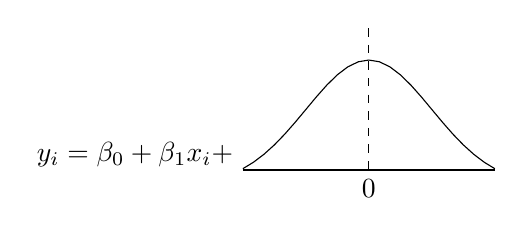
\begin{tikzpicture}[xscale = 0.8, yscale = 4]
		\coordinate (A) at (-2,0);
		\draw (A) node[left] {$y_i = \beta_0 + \beta_1 x_i + $};
		\draw [domain=-2:2] plot(\x, {exp((-(\x)^2)/2)/(sqrt(2*pi))-0.1});
		\draw [dashed] (0,0.4)--(0,-0.05);
		\draw (-2,-0.05)--(2,-0.05);
		\node (zero) at (0,-0.05)[below]{$0$};
	\end{tikzpicture}
\end{center}


% さて，この「確率的でないところ」が確率分布の中に入り込むとしたら，誤差$e_i$の平均値を一定の量，$\beta_0 + \beta_1 x_i$分だけ動かすことになります。
Now, if this "non-probabilistic part" enters the probability distribution, it means moving the average value of the error $e_i$ by a certain amount, $\beta_0 + \beta_1 x_i$.
% 回帰直線が表しているのは，誤差のない予測の線でもあります。実際のデータはそれに誤差が伴って生じます。確率モデルになった線形モデルは，図\ref{fig::24_01}のようなイメージで考えるといいかもしれません。
The regression line represents a line of error-free prediction. Actual data is generated with some errors. The linear model, now a probabilistic model, can be thought of in the same way as shown in Figure \ref{fig::24_01}.
\begin{figure}[ht]
   \centering
   \includegraphics[keepaspectratio,width=0.8\linewidth]{../images/24_ML/Rplot24_06.png}
   \caption{Error clinging to the predicted line}
   \label{fig::24_01}
\end{figure}


% ここで正規分布がもつ2つのパラメータ，$\mu$と$\sigma$は，それぞれ\textbf{位置}と\textbf{幅}を表しているわけですが，確率的でないところはこの位置をズラすような作用をすることになります。
Here, the two parameters that the normal distribution has, $\mu$ and $\sigma$, each represent \textbf{position} and \textbf{width}, respectively. If it is not stochastic, it will act to shift this position.

% 大事なところなので，もう一度式で確認しながら説明します。まず今回のモデルに含まれる情報は次のとおりです。
Since it's important, I'll explain again while checking with the formula. The information included in the model this time is as follows.
\begin{eqnarray}
   \hat{y}_i = \beta_0 + \beta_1 x_i \label{eq24_01}\\
   y_i = \hat{y}_i + e_i \label{eq24_02}\\
   e_i \sim N(0,\sigma)\label{eq24_03}
\end{eqnarray}

% ここで式\ref{eq24_01}と\ref{eq24_02}を合わせて，
Combine equations \ref{eq24_01} and \ref{eq24_02} here.
\begin{equation}
	\begin{array}{ccc}
		y_i & =    & \beta_0 + \beta_1 x_i +e_i \\
		e_i & \sim & N(0,\sigma)
	\end{array}
	\label{eq24_04}
\end{equation}

% とします。ここで$e_i$の中心は$0$で，それに$\beta_0 + \beta_1 x_i$が加わるのですから，
So here, the center of $e_i$ is $0$, and $\beta_0 + \beta_1 x_i$ is added to it.
\[ y_i \sim N(\beta_0 + \beta_1 x_i, \sigma) \]
ということになります。

あるいは，式\ref{eq24_02}と\ref{eq24_03}から先に，
\begin{eqnarray}
	\hat{y}_i &=& \beta_0 + \beta_1 x_i \label{eq24_05}\\
	y_i &\sim& N(\hat{y}_i,\sigma) \label{eq24_06}
\end{eqnarray}
と考えて，この式\ref{eq24_06}の$\hat{y}_i$に式\ref{eq24_05}を代入しても，
\[ y_i \sim N(\beta_0 + \beta_1x_i, \sigma) \]
% が得られます。どちらのルートでも結構ですから，自分のわかりやすい方で理解してください。一覧の流れを図\ref{m24_two_way_root}にまとめてみました。
You can get it. Either route is fine, so please understand it in the way that is easier for you. I tried to summarize the flow of the list in Figure \ref{m24_two_way_root}.
\begin{eqnarray}
   \hat{y}_i &=& \beta_0 + \beta_1 x_i \label{eq24_05}\\
   y_i &\sim& N(\hat{y}_i,\sigma) \label{eq24_06}
\end{eqnarray}

Translated:

The first line represents the estimated value of y for observation i. The second line states that the true value of the response variable y for observation i is normally distributed with mean equal to the estimated value and standard deviation equal to σ.



% これが回帰分析の\keytermL{確率モデル}{かくりつもでる}になります。
This becomes the probability model of regression analysis.
% ポイントは，確率分布の位置を表すパラメータに，数式で表現された\textbf{構造}を書き込んだところにあります。狭義の\textbf{モデリング}とは，確率分布のパラメータに構造を与えるもの，ということができるでしょう。
The point lies in writing a mathematical representation of the \textbf{structure} into the parameter that represents the position of the probability distribution. In a strict sense, \textbf{modeling} could be defined as giving a structure to the parameters of the probability distribution.
% 発展的な話題になりますが，正規分布に限らず\keytermL{ベルヌーイ分布}{べるぬーいぶんぷ}や\keytermL{二項分布}{にこうぶんぷ}，\keytermL{ポアソン分布}{ぽあそんぶんぷ}などのパラメータを数式で表現したモデルを考えることもできます。正規分布以外の確率分布でパラメータに線形モデルを与えたものを\keyterm{一般化線形モデル}{いっぱんかせんけいもでる}{Generalized Linear Model}と呼びます\footnote{\keyterm{一般線形モデル}{いっぱんせんけいもでる}{General Linear Model}($\to$セクション\ref{GeneralLinearModel},Pp.\pageref{GeneralLinearModel})と混同しないように注意してください。}。一般化線形モデルになると，比率や度数などより広い範囲のデータを扱う分析ができるようになります\footnote{本学では二年次選択科目のデータ解析応用で扱います。興味がある人，履修をお待ちしています。}。
The subject will become more advanced, but not only the normal distribution, but also models that express parameters in mathematical formulas such as the Bernoulli distribution, the binomial distribution, and the Poisson distribution can be considered. Things that give a linear model to parameters in a probability distribution other than the normal distribution are called generalized linear models. Please be careful not to confuse it with the general linear model (Refer to section\ref{GeneralLinearModel},Pp.\pageref{GeneralLinearModel}). When it becomes a generalized linear model, you will be able to analyze a wider range of data such as ratios and frequencies. This subject is covered in the optional course of data analysis application in the second year of our school. We look forward to those who are interested in enrolling.

% \section{確率モデルの最尤推定}
\section{Maximum Likelihood Estimation of Probability Models}

% このようにして確率モデルを書くことができれば，あとはこれにしたがって「データがこの確率モデルから出てくる尤もらしさが最も高くなるように，未知パラメータを推定すれば良いということになります。
If you can write a probability model like this, then all you have to do is "estimate the unknown parameters so that the likelihood of the data coming from this probability model is maximized".
% 改めて確認ですが，今回のモデル$y_i \sim N(\beta_0 + \beta_1x_i, \sigma)$において未知な数字は$\beta_0,\beta_1,\sigma$の3つになります。
To confirm once again, in our model $y_i \sim N(\beta_0 + \beta_1x_i, \sigma)$, the unknown numbers are the three ($\beta_0$, $\beta_1$, $\sigma$).


% 正規分布の式をちゃんと書くと，$x$という値が出てくる確率密度は
When properly writing the formula for a normal distribution, the probability density for a value $x$ to occur is
\[ p(x) = \frac{1}{\sqrt{2\pi \sigma}}exp\left( - \frac{(x-\mu)^2}{2\sigma^2}\right)\]
となります。この平均$\mu$のところに$\beta_0 + \beta_1 x_i$という数式を入れることになります。

すでに入り組んだ形をしているので，イメージしづらいところがあるかもしれませんが，あるデータ$y_i$が得られる確率密度は
\[ p(y_i) = \frac{1}{\sqrt{2\pi \sigma}}exp\left( -\frac{(y_i-\mu)^2}{2\sigma^2}\right)\]
% ですから，$\mu=\hat{y_i} = \beta_0 + \beta_1 x_i$を代入して
Therefore, substitute $\mu=\hat{y_i} = \beta_0 + \beta_1 x_i$
\[ p(y_i) = \frac{1}{\sqrt{2\pi \sigma}}exp\left( -\frac{(y_i-\beta_0 - \beta_1 x_i)^2}{2\sigma^2}\right)\]
となります。

データは$i = 1,2,\cdots,N$とあり，それらが同じ母集団から独立に得られている，と考えます(i.i.d.)。つまり手元に同時にこれらのデータが出揃うときの尤度$L$は，上記の確率密度($p(y_i)$)を全部掛け合わせたもの\footnote{コインが表，表，裏，と出たら$\theta \times \theta \times (1-\theta)$と欠けたことを思い出して！}，と考えることができますね。
$i$を$1$から$n$まで足し合わせることを総和する，といって$x_1+x_2+\cdots+x_N=\sum_{i=1}^N x_i$と表しますが，同様にすべて掛け合わせる総積は，
\[ x_1 \times x_2 \times \cdots x_N = \prod_{i=1}^N x_i \]
% と書きます。ここでの記号$\prod$は\ruby{総積}{プロダクト}と言いますが，これを使って尤度$L(Y_i)$を表現すると，次のようになります。
It says, "Here, the symbol $\prod$ is called a product. When using this to express the likelihood $L(Y_i)$, it can be represented as follows."

\[ L(y_i | \beta_0,\beta_1,\sigma) = \prod_{i=1}^N \frac{1}{\sqrt{2\pi \sigma}}exp\left(- \frac{(y_i-\beta_0 - \beta_1 x_i)^2}{2\sigma^2}\right)\]

ここで$L(y_i | \beta_0,\beta_1,\sigma) $という書き方の，$\mid$は何かというと，この縦線の右側にある$\beta_0,\beta_1,\sigma$が与えられた場合の，という条件付き確率の書き方を借りた\keyterm{尤度}{ゆうど}{Likelihood}を表しています。

さてこれは確率(密度)の掛け算になりますから，すごく小さな数字になって実際の計算は大変です。そこで前回習ったように，尤度そのものではなく\keyterm{対数尤度}{たいすうゆうど}{log-likelihood}をとって，その最大値を求めるということにしたいと思います。対数をとると掛け算は足し算に変わりますから，$\prod \to \sum$に記号が変わりまして，対数尤度の関数は次のようになります。

\[ \log L(y_i | \beta_0,\beta_1,\sigma) = \sum_{i=1}^N \log \left[ \frac{1}{\sqrt{2\pi \sigma}}exp\left( -\frac{(y_i-\beta_0 - \beta_1 x_i)^2}{2\sigma^2}\right)\right]\]

% 非常に面倒な形をしていますね！しかもこれは$\beta_0,\beta_1,\sigma$という3つの変数が同時に関わりますから，連立微分方程式を解くことになります。
It has a very complicated shape! Moreover, this involves three variables $\beta_0,\beta_1,\sigma$ simultaneously, so it will require solving a system of differential equations.
% でももちろん大丈夫。この面倒な計算は，Rがやってくれますから私たちはなんの心配もする必要はありません。
But of course, it's fine. Since R does this troublesome calculation for us, there's no need for us to worry at all.

% しかもこの最尤推定の結果得られる$\beta_0,\beta_1$の値は，\underline{最小二乗法の結果と一致}します。
Moreover, the values of $\beta_0, \beta_1$ obtained as a result of this maximum likelihood estimation \underline{match the results of the least squares method}.
% ですから，実質的にはただの回帰分析をすれば良いのです。
Therefore, in essence, all we need to do is perform a simple regression analysis.

% \subsection{実践例}
\subsection{Practical Example}
% 数字としてはなんら変わるところはないのですが，復習も兼ねて第\ref{m09_Regression}講でやった回帰分析をもう一度見てみましょう。
There is no change in terms of numbers, but let's take another look at the regression analysis we did in lecture \ref{m09_Regression} for review purposes.
% 回帰分析の関数は\verb|lm|という関数名で，Rがデフォルトで持っている関数なのでした。実はこの関数，最尤推定値を返す関数だったのです。
The regression analysis function is named \verb|lm|, a function that R has by default. In fact, this function was one that returns the maximum likelihood estimates.
% そのときは\keytermL{最小二乗法}{さいしょうにじょうほう}の説明しかしていなかったのですが，関数の使い勝手のこともあって，最尤推定する関数でご紹介しておりました。
At that time, I only explained the least squares method, but considering the usability of the function, I introduced it with the maximum likelihood estimation function.
% 本当の意味で，最小二乗法のアルゴリズムで回帰分析をするときは\verb|lsfit|関数というものを使います。
In the true sense, when doing regression analysis with the least squares method algorithm, we use a function called \verb|lsfit|.

% 使用例をコード\ref{code:24_01}に示しました。ここでは野球選手のデータを使って，身長から体重を予測するというモデルを実行しています\footnote{第\ref{m11_MRonR}講と同じ分析結果です。}。
The usage example is shown in code \ref{code:24_01}. Here we are running a model to predict weight from height using data from baseball players\footnote{This is the same analysis result as in lecture \ref{m11_MRonR}.}.
\begin{lstlisting}[language=c++,label={code:24_01},caption={二つの推定法の比較}]
# 最小二乗法の推定
result.LS <- lsfit(x = batter$height, y = batter$weight)
result.LS$coefficients
# 最尤推定
result.LM <- lm(weight ~ height, data = batter)
result.LM
\end{lstlisting}

% 結果は出力\ref{RS:out24_01}のようになります。
The result will look like output \ref{RS:out24_01}.
\begin{lstlisting}[language=c++,label={code:24_01},caption={Comparison of Two Estimation Methods}]
# Least Squares Estimation
result.LS <- lsfit(x = batter$height, y = batter$weight)
result.LS$coefficients
# Maximum Likelihood Estimation
result.LM <- lm(weight ~ height, data = batter)
result.LM
\end{lstlisting}


% これを見ると明らかなように，どちらの方法でやっても同じ推定値(切片$\beta_0=-124.918$，傾き$\beta_1=1.167$)になっていますね。また少し余談ではありますが，最尤推定した結果の最終行を見ると，$F$統計量が自由度$F(1,327)=226.9$とあり，この$p$値も計算されています。ここで線形モデルと要因計画・帰無仮説検定も関連があることがわかります\footnote{ここでは切片以外のすべての説明変数(今回の例では単回帰なので説明変数は一つですが)の傾きが0である，という帰無仮説にたいして検定が行われています。}。
As you can see when looking at this, whether done in either way, we get the same estimated value (intercept $\beta_0=-124.918$, slope $\beta_1=1.167$). Also, although it's bit of a digression, if you look at the last line of the maximum likelihood estimation result, you'll see that the $F$ statistic is degrees of freedom $F(1,327)=226.9$, and this $p$-value is also calculated. From this, it's understood that there is a connection between the linear model, factorial plans, and null hypothesis tests\footnote{Here, a test is being done against the null hypothesis that all slopes of explanatory variables (other than intercept, which, in this case, since it's a simple regression, there is only one explanatory variable) are zero.}.

% 方法が違っても推定値が同じ，というのは前回もお話ししたように，同じ母数を推定しているわけですからむしろ当然の結果です。1つの山の頂上に達するのに，複数のルートがあってもゴールは同じ，ということです。
Although the methods may be different, it is natural that the estimates are the same, as we discussed previously, because they are estimating the same parameter. It's like reaching the top of a mountain, the goal is the same even if there are multiple routes.
% 違う点があるとすれば，最尤推定の場合は誤差の標準偏差$\sigma$も推定されているというところでしょうか。結果に$\sigma=...$という記載はありませんが，よく見ると\verb|Residuals|のところに残差$e$の最小値，最大値，四分位偏差，中央値などが示されており，誤差が分布するものと考えられていることがわかります。
If there's a difference, it would be that in the case of maximum likelihood estimation, the standard deviation of the error $\sigma$ is also estimated. There is no notation in the results such as $\sigma=...$, but if you look closely, you can see the minimum, maximum, quartile deviation, and median of the residual $e$ in the \verb|Residuals| section, suggesting that the error is considered to be distributed.

% 今回は説明変数が1つの単回帰分析でしたが，説明変数の数が増えた\keyterm{重回帰分析}{じゅうかいきぶんせき}{Multiple Regression Analysis}でも同じで，\verb|lm|関数はデータが正規分布から得られたものとした上で，尤度を最大にする推定値を返してくれます。
This time we performed a simple regression analysis with one explanatory variable, but the same applies to multiple regression analysis when the number of explanatory variables increases. The `lm` function returns the estimate that maximizes the likelihood, assuming that the data is obtained from a normal distribution.

% 今のところ，最小二乗法と最尤法，結局答えが同じになるのに，なぜこんな回りくどい話をするのかと思うかもしれません。
You might be wondering why we're having such a roundabout discussion when in the end, the answers will be the same with both the least squares method and the maximum likelihood method.
% 大事なのは線形モデルが確率モデルになったというところで，確率モデルになることで適用できる範囲が広がるから，というのが1つの答えです。
The important thing is that the linear model has become a probabilistic model, and the fact that it has become a probabilistic model has broadened the range where it can be applied - this is one answer.
% ところがもう1つ大事なことがあるのです。それは次回以降，第三の母数推定法である\keyterm{ベイズ法}{べいずほう}{Bayesian estimation method}に関係します。実はこの第三の方法も確率モデルを使ったものなのですが，詳しくは次回の講釈で。
However, there is one more important thing. It relates to the Bayes method, the third parameter estimation method, in the future. Actually, this third method also uses a probability model, but I will elaborate on it in the next lecture.


% \section{課題}
\section{Problem}
% \paragraph{回帰分析の結果を読み取る}出力\ref{RS:out24_01}の読み取り方について，正しい記述をすべて選んでください。
\paragraph{Interpreting Regression Analysis Results} Please select all the correct descriptions about how to read output \ref{RS:out24_01}.
Translation:

\begin{Rscreen}{Comparison Result}{out24_01}
   \begin{verbatim}
> # Estimation by least squares method
> result.LS <- lsfit(x = batter$height, y = batter$weight)
> result.LS$coefficients
  Intercept           X 
-124.917552    1.166698 
> # Maximum likelihood estimation
> result.LM <- lm(weight ~ height, data = batter)
> summary(result.LM)

Call:
lm(formula = weight ~ height, data = batter)

Residuals:
     Min       1Q   Median       3Q      Max 
-20.9217  -4.9213  -0.4214   4.0783  28.9118 

Coefficients:
              Estimate Std. Error t value Pr(>|t|)    
(Intercept) -124.91755   13.89317  -8.991   <2e-16 ***
height         1.16670    0.07746  15.063   <2e-16 ***
---
Signif. codes:  0 ‘***’ 0.001 ‘**’ 0.01 ‘*’ 0.05 ‘.’ 0.1 ‘ ’ 1

Residual standard error: 7.435 on 327 degrees of freedom
Multiple R-squared:  0.4096,	Adjusted R-squared:  0.4078 
F-statistic: 226.9 on 1 and 327 DF,  p-value: < 2.2e-16
    \end{verbatim}
\end{Rscreen}

\end{document}
